% =============================================================
% ChIP-seq Assignment Report — Overleaf-ready
% Compile: pdflatex report.tex   (or LuaLaTeX/XeLaTeX)
% Place igv.png in the same directory.
% =============================================================
\documentclass[11pt,a4paper]{article}

\usepackage[a4paper,margin=2.2cm]{geometry}
\usepackage{graphicx}
\usepackage{booktabs}
\usepackage{microtype}
\usepackage{hyperref}
\usepackage{caption}
\usepackage{xcolor}
\usepackage{titlesec}
\usepackage{amsmath}

\titleformat{\section}{\normalfont\normalsize\bfseries}{\thesection}{0.5em}{}
\setlength{\parskip}{3pt}
\setlength{\parindent}{0pt}

\hypersetup{colorlinks=true,linkcolor=blue!50!black,urlcolor=blue!50!black}

% -- Front matter —
\newcommand{\studentname}{Aryaman Bahl}
\newcommand{\studentid}{2022113010}
\newcommand{\coursecode}{Molecular Biology — S26}
\newcommand{\submissiondate}{\today}

% -- Resources —
\newcommand{\repourl}{https://github.com/hanara2112/chipseq.git}
\newcommand{\notebookurl}{https://hanara2112.github.io/chipseq/docs/extra_enhancer_analysis.html}

\title{\vspace{-2em}\textbf{H3K27ac ChIP-seq in IL7-High Mouse T-cells:\\[-0.3em]
Active Enhancer Landscape Profiling vs IgG Background}}
\author{\studentname\ \textbar\ \studentid\ \textbar\ \coursecode}
\date{\vspace{-0.8em}\submissiondate}

\begin{document}
\maketitle

\begin{center}\normalsize
\href{\repourl}{\texttt{Code}}\ \textbar\ 
\href{\notebookurl}{\texttt{Notebook}}
\end{center}

% =============================================================
\section*{Introduction}
Histone modifications form a major regulatory layer of the genome. Two of the most informative are H3K4me3 and H3K27ac. \textbf{H3K4 trimethylation} is added at active transcription start sites (TSSs) by the COMPASS/SET1 complex and marks active \emph{promoters}. \textbf{H3K27 acetylation} is added by p300/CBP and marks both active promoters and active distal \emph{enhancers}. Mapping these two marks therefore gives a readout of which regulatory elements are turned on in a given cell state.

The data analysed in this report are an H3K27ac ChIP library (sample S295) and a matched IgG control (sample S286) from IL-7-stimulated mouse T-cells, each $\approx\!10^{6}$ read pairs against mm10. The goal is to call regions of H3K27ac enrichment, show they sit well above the IgG background, describe where they fall in the genome, and connect those locations back to promoter and enhancer biology.

% =============================================================
\section*{Methods (brief)}
Reads were quality-checked (FastQC/MultiQC), adapter- and quality-trimmed (Trim~Galore at $Q\!\geq\!20$), and aligned to mm10 with Bowtie2 in paired-end mode. Aligned BAMs were de-duplicated, then filtered to retain only properly-paired alignments with $\text{MAPQ}\!\geq\!20$. H3K27ac peaks were called with MACS2 in broad-peak mode using the IgG library as control; strong cores were called at $q\!\leq\!0.05$ and weaker bridge regions joining them at $q\!\leq\!0.10$, as is standard for broad histone marks in MACS2. An IgG self-call (no control) provided a negative-control baseline. Peaks were annotated to genomic features with ChIPseeker against \texttt{TxDb.Mmusculus.UCSC.mm10.knownGene}, and RPKM-normalised coverage tracks were visualised in IGV. Detailed parameters and tool versions are deposited alongside the code (see \emph{Resources}).

% =============================================================
\section*{Results}

\subsection*{Read quality, alignment, and post-processing}
All four FASTQ files passed per-base sequence quality QC: median Phred scores were $\geq$30 across all 151\,bp positions in every sample, with no detectable 3$'$-end quality decay. Both libraries flagged the expected presence of Illumina TruSeq adapter sequence, which was successfully removed by trimming; the IgG library additionally showed a slightly broader GC distribution than the H3K27ac sample (41--43\,\% vs.\ 51\,\%), consistent with IgG sampling the genome more uniformly while a specific antibody enriches for GC-biased regulatory regions. Adapter removal is essential because adapter bases are not present in the reference genome and would otherwise either prevent alignment or cause artefactual signal at read ends.

Bowtie2 aligned 95.80\,\% of S295 reads and 95.33\,\% of S286 reads to mm10 (Table~\ref{tab:pipeline}). The fraction of \emph{concordantly and uniquely} mapped pairs — meaning both mates align to the same chromosome in the expected orientation, within the expected fragment size, and to a single best location — was 88.26\,\% for S295 versus 74.44\,\% for S286. The lower unique-mapping fraction of IgG reflects its non-specific nature: it samples repetitive sequence proportionally to its genomic abundance, and reads from repeats cannot be uniquely placed. The remaining $\sim$5\,\% of unaligned reads in each library are typical and arise from residual adapter dimers, sequencing errors, contamination, and reads from regions absent or collapsed in the reference. Capping the maximum allowed insert size at 2\,kb during alignment prevents Bowtie2 from spuriously pairing reads that map far apart due to structural variation or random ligation artefacts, while still being permissive of all biologically real ChIP fragments (typically 200--500\,bp after sonication).

PCR duplicates — read pairs with identical mapping coordinates that originate from a single template molecule over-amplified during library preparation — inflate apparent coverage at specific positions and produce sharp false peaks if not removed. Duplication rates after marking (with mate-information first reconstructed by a fixmate step, which is required for paired-end duplicate identification) were healthy at 8.14\,\% (S295) and 9.74\,\% (S286), within the $<$15\,\% range expected for a complex library. The slightly higher IgG rate is consistent with its smaller pool of unique fragments being amplified more deeply. A subsequent quality filter retained only properly-paired alignments with $\text{MAPQ}\!\geq\!20$. The MAPQ score is a Phred-scaled estimate of the probability that a read is mis-placed; a threshold of 20 corresponds to a 1\,\% mis-mapping ceiling and is the standard cutoff because it removes effectively all multi-mappers (which carry MAPQ\,0--1) while retaining most high-confidence unique alignments. Reads of low MAPQ are dominated by repetitive elements (SINEs, LINEs, satellites), segmental duplications, centromeric and pericentromeric regions, and recently duplicated paralogous gene families.

\begin{table}[h]
\centering
\caption{Read flow through the processing pipeline. All counts are paired-end read pairs.}
\label{tab:pipeline}
\small
\begin{tabular}{lrr}
\toprule
Step & S295 (H3K27ac) & S286 (IgG) \\
\midrule
Raw read pairs                              & 998{,}581 & 998{,}498 \\
Bowtie2 overall alignment rate              & 95.80\,\%  & 95.33\,\%  \\
\;\;Concordant, unique                      & 88.26\,\%  & 74.44\,\%  \\
\;\;Concordant, multi-mapper                & 7.54\,\%   & 20.89\,\%  \\
PCR duplicate rate                          & 8.14\,\%   & 9.74\,\%   \\
Pairs after duplicate removal               & 917{,}282 & 901{,}333 \\
Pairs after MAPQ\,$\geq$\,20 + proper-pair  & 830{,}371 & 730{,}724 \\
\bottomrule
\end{tabular}
\end{table}

\subsection*{Peak calling: ChIP versus IgG}
A peak in ChIP-seq is a contiguous genomic interval where the local density of immunoprecipitated reads is statistically elevated above the surrounding background — operationally, a region the antibody has bound repeatedly, indicating local enrichment of the targeted modification. A matched control such as an IgG library is necessary because background read density is not uniform across the genome: chromatin accessibility, sonication bias, GC-content effects, and non-specific antibody pull-down all produce regional pile-ups that have nothing to do with the histone mark. MACS2 distinguishes real enrichment from such noise by modelling the local read distribution under a dynamic Poisson whose mean is taken from the control track over multiple length scales (1\,kb, 5\,kb, 10\,kb), computing a $p$-value at every position, and controlling the false-discovery rate by Benjamini--Hochberg adjustment.

Run in broad-peak mode against the IgG control (strong cores at $q\!\leq\!0.05$, weak bridge regions at $q\!\leq\!0.10$), MACS2 returned \textbf{18{,}681} significantly enriched H3K27ac regions (Table~\ref{tab:peaks}). Peaks have a median width of 1{,}218\,bp (max 27\,kb) and a mean fold-enrichment of 4.54$\times$ over IgG (max 17.12$\times$); the ten strongest peaks span 13--17$\times$ enrichment and lie on autosomes only — collectively a clean, broad active-chromatin signature with the multi-nucleosomal width expected of H3K27ac. The IgG self-call, run with no control at the identical statistical threshold, returned \textbf{zero} peaks. This is the ideal outcome: it demonstrates that the IgG library has no locus-specific enrichment of its own, and therefore that the 18{,}681 H3K27ac peaks cannot be explained by chromatin accessibility, sonication bias, or PCR artefacts — they reflect genuine antibody-driven enrichment for the targeted modification. As an additional quality check, 66.3\,\% of all H3K27ac reads fall inside a called peak (the ``fraction of reads in peaks'' metric), far above the 1\,\% minimum recommended for a usable ChIP-seq library.

\begin{table}[h]
\centering
\caption{Peak count summary (MACS2, $q\!\leq\!0.05$).}
\label{tab:peaks}
\small
\begin{tabular}{lllr}
\toprule
Sample & Mark & Mode & \# Peaks \\
\midrule
S295 (H3K27ac) & H3K27ac      & broad, IgG-controlled & \textbf{18{,}681} \\
S286 (IgG)     & IgG control  & narrow, no control    & \textbf{0}        \\
\bottomrule
\end{tabular}
\end{table}

\subsection*{Genomic distribution of peaks}
Annotation of the 18{,}681 peaks against mm10 gene models (TSS region $\pm$3\,kb) produced the distribution: \textbf{55.34\,\%~promoter} (50.5\,\% within 1\,kb of a TSS, 2.3\,\% within 1--2\,kb, and 2.6\,\% within 2--3\,kb), \textbf{18.82\,\%~distal intergenic}, \textbf{18.08\,\%~intronic} (1\textsuperscript{st} and other introns combined), and 8.05\,\%~exonic/UTR. The promoter share captures the well-described co-occurrence of H3K27ac and H3K4me3 at \emph{actively transcribing} promoters; the combined intronic + distal-intergenic share ($\sim$37\,\%) corresponds to the canonical pool of distal active enhancers that H3K27ac additionally marks. Enhancers appear far from gene promoters because they are \emph{cis}-regulatory elements that contact their target promoter through cohesin/CTCF-anchored 3D chromatin loops — they are not constrained to lie next to the gene they regulate, and most often live tens of kilobases away in introns of the regulated gene or in distal intergenic space.

It is worth noting that the promoter share recovered here is somewhat higher than canonical literature values for H3K27ac in mammalian cells (typically 30--40\,\% promoter). Two technical effects most likely contribute: (i) in broad-peak mode, a peak that overlaps a TSS even partially is classified entirely as ``Promoter'' regardless of where the bulk of the signal lies, which inflates the promoter bin relative to what a narrow caller would report; and (ii) at the shallow $\approx\!10^{6}$ read-pair sequencing depth, the peaks recovered are preferentially the strongest in the genome, which are concentrated at active promoters where H3K4me3 and H3K27ac co-occur.

\subsection*{Coverage visualisation in IGV}
Figure~\ref{fig:igv} shows the RPKM-normalised IGV coverage tracks for the H3K27ac and IgG libraries together with the called peak annotation. Peak height in the browser represents read coverage depth at that position (here RPKM-normalised), so taller peaks correspond to more sequenced fragments stacked at the locus and therefore more H3K27ac-modified chromatin pulled down by the antibody. Three observations are immediately visible: (i) the H3K27ac track shows a discrete, broad domain that overlaps the MACS2 peak interval; (ii) the IgG track on the same axis is essentially flat across the same window, mirroring the quantitative observation that IgG produced zero peaks genome-wide; and (iii) the H3K27ac peak is visibly broad — were an H3K4me3 track loaded at the same locus it would appear as a much sharper, narrower spike, because H3K4me3 is deposited on a small number of nucleosomes immediately flanking the TSS, while H3K27ac decorates the entire body of an active enhancer or promoter, often spanning tens of nucleosomes.

\begin{figure}[h]
\centering
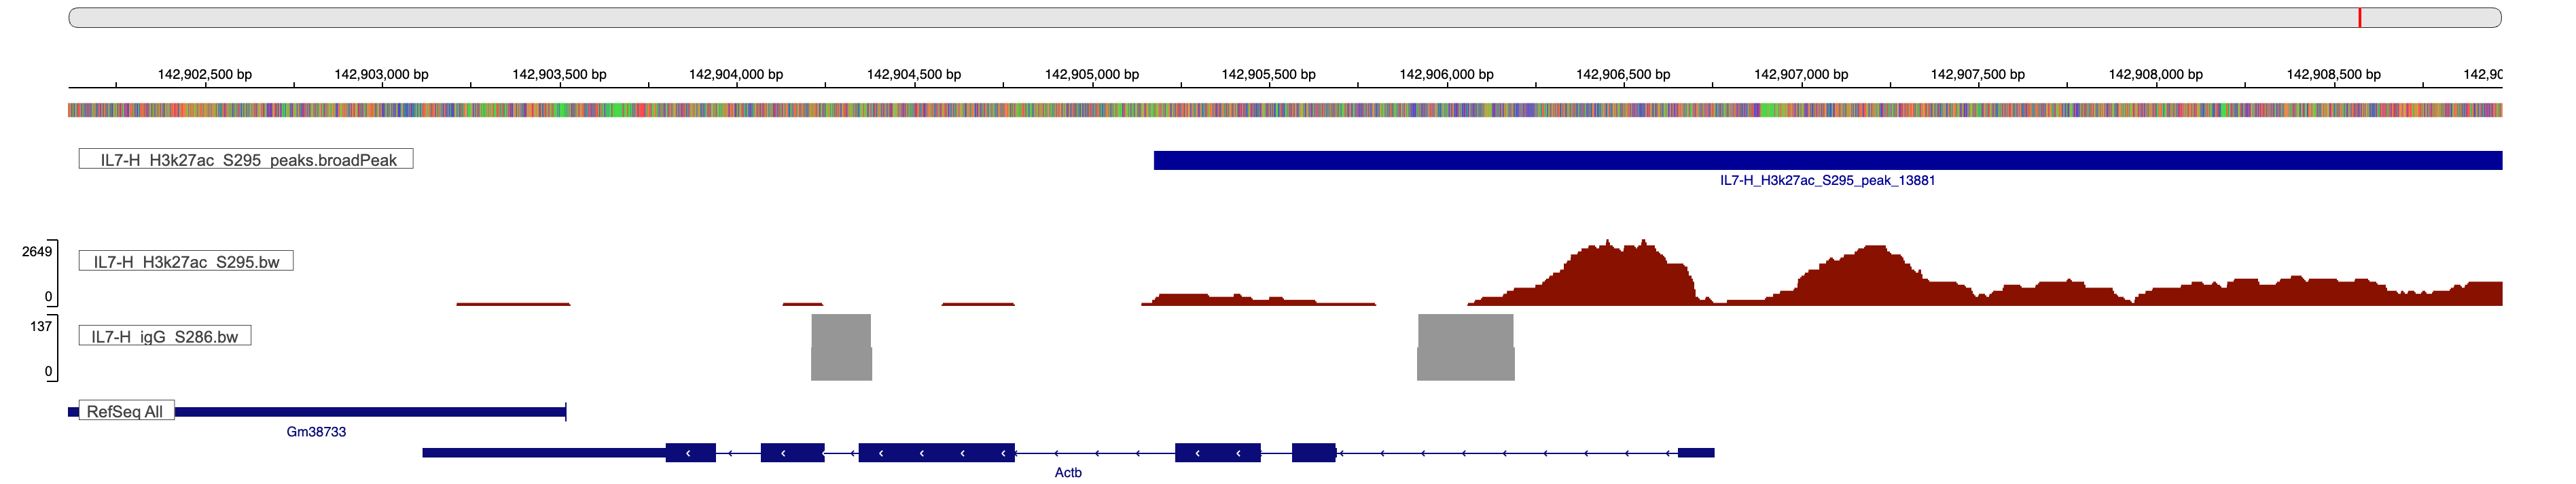
\includegraphics[width=0.95\linewidth]{igv.png}
\caption{Representative IGV view at \textbf{Actb 
  (chr5:142{,}901{,}500--142{,}904{,}600)}. Top: H3K27ac (S295) RPKM coverage showing a broad pile-up over the called peak. Bottom: IgG (S286) RPKM coverage on the same locus, flat. The peak interval shown is one of the strongest H3K27ac peaks (fold-enrichment $>$13$\times$ over IgG).}
\label{fig:igv}
\end{figure}

% =============================================================
\section*{Biological interpretation}
The genes nearest the strongest H3K27ac peaks make biological sense for IL-7-stimulated T-cells. Two of the top ten peaks lie at the promoters of \emph{Ep300} — the very enzyme that writes the H3K27ac mark — and \emph{Ptprcap}, a regulator of T-cell receptor signalling. Looking across all 18{,}681 peaks, a Gene Ontology over-representation test on the associated genes returned cell-cycle and proliferation processes as the strongest hits (\emph{mitotic cell cycle phase transition}, \emph{chromosome segregation}, \emph{DNA replication}; q\,$\approx$\,0). This is the expected signature for IL-7, which is the canonical lymphocyte proliferation cue, and provides an independent biological check that the peak set reflects real chromatin biology.

The results also define two complementary populations of H3K27ac signal in IL-7-stimulated T-cells. The promoter-proximal majority ($\sim$55\,\% of peaks) identifies the set of actively transcribing genes in this cell state — a snapshot of the current transcriptional programme. Where this overlaps an H3K4me3 promoter set (not assigned to this report) it would mark fully active genes, distinct from \emph{bivalent} loci that carry only H3K4me3 and are transcriptionally poised. The remaining $\sim$37\,\% of peaks at intronic and distal-intergenic positions identifies the active enhancer landscape of the cell. Active enhancers are the principal determinants of cell identity: housekeeping promoters are largely shared across tissues, but each cell type marks a unique subset of enhancers with H3K27ac, and remodelling that enhancer set — for example in response to IL-7 signalling, where STAT5 is the canonical downstream effector and lineage transcription factors act in parallel — is how T-cells reshape their gene-expression programme. Loss of an enhancer's H3K27ac, e.g.\ via inhibition of p300 or BRD4, collapses transcription of the connected gene without altering the promoter itself, illustrating the causal regulatory role of these distal sites.

The two histone marks studied in this assignment occupy complementary positions within this picture. H3K4me3 is geometrically restricted to active TSSs because it is deposited by COMPASS/SET1 in tight association with the RNA Pol II pre-initiation complex and feeds back to recruit TFIID via the PHD finger of TAF3 — it is in effect a local stabiliser of the transcription-permissive state at gene starts, producing narrow, focused peaks. H3K27ac, by contrast, is laid down by p300/CBP at any chromatin region engaged by transcription factors and co-activators, and so spreads broadly along enhancer bodies that may lie far from any annotated TSS. The genomic distribution observed here — 55\,\% promoter / 19\,\% intergenic / 18\,\% intronic — sits exactly between the textbook profile of a pure promoter mark and that of a pure enhancer mark, faithfully reflecting H3K27ac's dual role at both active promoters and active enhancers.

These chromatin modifications qualify as \emph{epigenetic} regulators because they satisfy the operational definition: they are heritable across DNA replication and cell division (writers re-deposit them on newly assembled nucleosomes), reversible by dedicated writer/reader/eraser enzymes (here p300/CBP and HDACs in the case of H3K27ac), and alter gene expression without altering the underlying DNA sequence. Together with DNA methylation and 3D chromatin architecture they encode the cellular memory that allows a single genome to support hundreds of stable, distinct cell states — and quantitative profiling of their genome-wide distribution, as performed here, is one of the most direct experimental windows onto that regulatory layer.

% =============================================================
\section*{Conclusion}
An H3K27ac ChIP-seq library from IL-7-stimulated mouse T-cells yielded \textbf{18{,}681} broad active-chromatin peaks against \textbf{zero} peaks in the matched IgG control. The peaks distribute as 55\,\% at promoters and 37\,\% at distal/intronic sites, recapitulating H3K27ac's dual role at both active promoters and active enhancers. The peak set passes independent quality checks (66\,\% of reads fall inside peaks; the strongest peaks include the \emph{Ep300} acetyltransferase locus itself and known T-cell signalling genes) and the associated gene set is enriched for cell-cycle and DNA-replication processes — exactly the biology IL-7 is known to drive in lymphocytes. The data therefore provide a clean, biologically validated map of active chromatin in this cell state.

% =============================================================
\section*{References}
\footnotesize
\begin{enumerate}\setlength\itemsep{0pt}
\item Andrews S. \textbf{FastQC}: a quality control tool for high-throughput sequence data. \emph{Babraham Bioinformatics}, 2010.
\item Krueger F. \textbf{Trim Galore}: a wrapper around Cutadapt and FastQC. \emph{Babraham Bioinformatics}.
\item Langmead B, Salzberg SL. Fast gapped-read alignment with \textbf{Bowtie 2}. \emph{Nat Methods} 9:357--359, 2012.
\item Danecek P et al. Twelve years of \textbf{SAMtools and BCFtools}. \emph{GigaScience} 10:giab008, 2021.
\item Zhang Y et al. Model-based Analysis of ChIP-Seq (\textbf{MACS}). \emph{Genome Biology} 9:R137, 2008.
\item Ramírez F et al. \textbf{deepTools2}: a next generation web server for deep-sequencing data analysis. \emph{NAR} 44:W160--W165, 2016.
\item Yu G, Wang LG, He QY. \textbf{ChIPseeker}: an R/Bioconductor package for ChIP peak annotation. \emph{Bioinformatics} 31:2382--2383, 2015.
\item Wu T et al. \textbf{clusterProfiler 4.0}: a universal enrichment tool for interpreting omics data. \emph{The Innovation} 2:100141, 2021.
\item Robinson JT et al. Integrative Genomics Viewer (\textbf{IGV}). \emph{Nat Biotechnol} 29:24--26, 2011.
\item Creyghton MP et al. Histone H3K27ac separates active from poised enhancers and predicts developmental state. \emph{PNAS} 107:21931--21936, 2010.
\end{enumerate}

\vspace{0.4em}
\noindent\textbf{Code \& data:} \href{\repourl}{\texttt{github.com/hanara2112/chipseq}} \; \textbar\; \textbf{Bonus notebook (live):} \href{\notebookurl}{\texttt{hanara2112.github.io/chipseq/.../extra\_enhancer\_analysis.html}}

\end{document}
